\documentclass[a4paper,12pt]{article}


\usepackage{setspace}
\usepackage{xcolor}
\usepackage{graphicx}
\usepackage{geometry}
\usepackage{float}
\usepackage{titlesec}
\usepackage{subfigure}
\usepackage{caption}
\captionsetup{figurewithin=section}
\usepackage{amsmath}
\usepackage{enumitem}
\usepackage{amssymb}
\usepackage{mathrsfs}


\begin{document}

\title{\textbf{Homework 1}}
\author{Yunian Pan}
\maketitle{}

\section{Problem 1: Overfitting}

Select some typical values of d from \{1, \ldots, 20\}, the fitting lines are shown as below:
\begin{figure}[htbp]
\setcounter{subfigure}{0}
\centering
\subfigure[d=1]{
\includegraphics[width = .45\textwidth]{1_1}
}
\subfigure[d=3]{
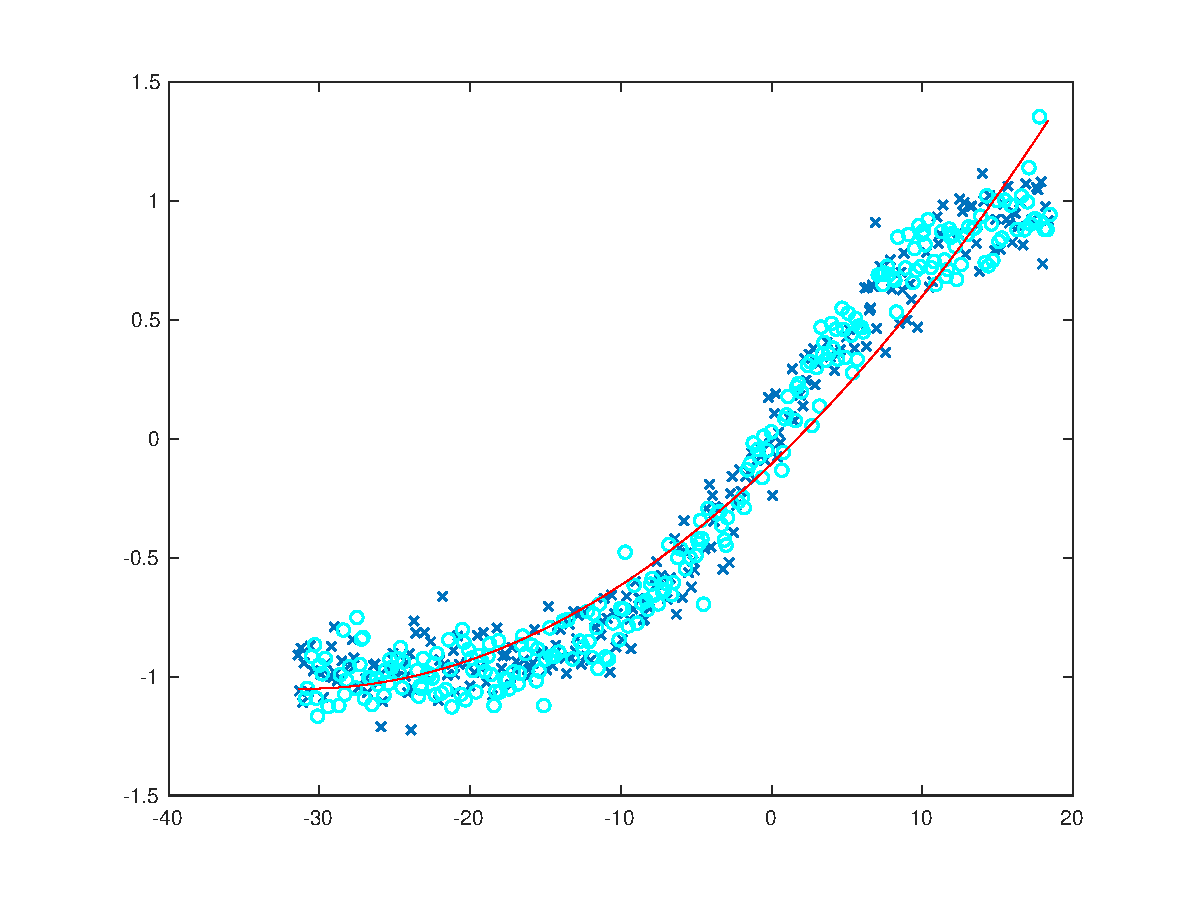
\includegraphics[width = .45\textwidth]{1_2}
}
\end{figure}
\\
\begin{figure}[htbp]
\centering
\subfigure[d=6]{
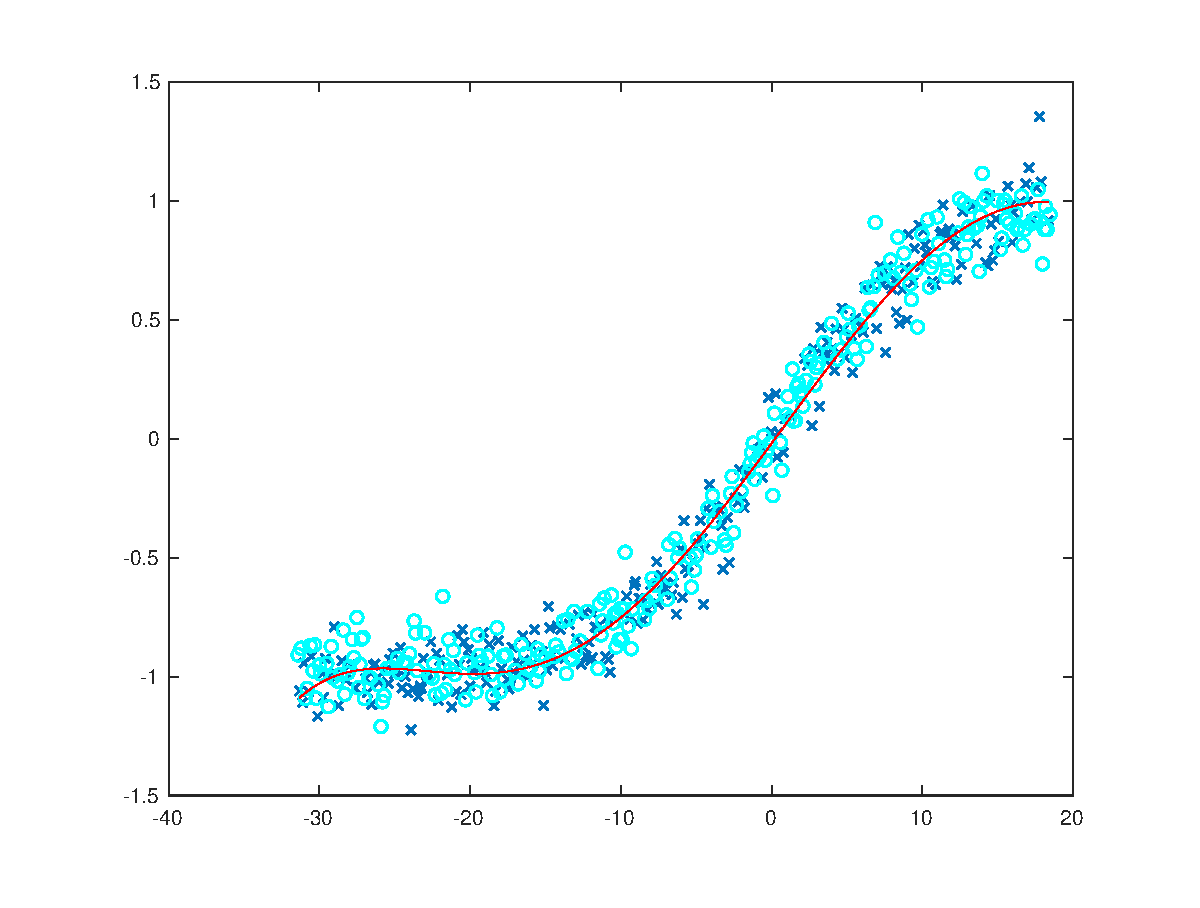
\includegraphics[width = .45\textwidth]{1_3}
\label{Fig.sub.1}
}
\subfigure[d=9]{
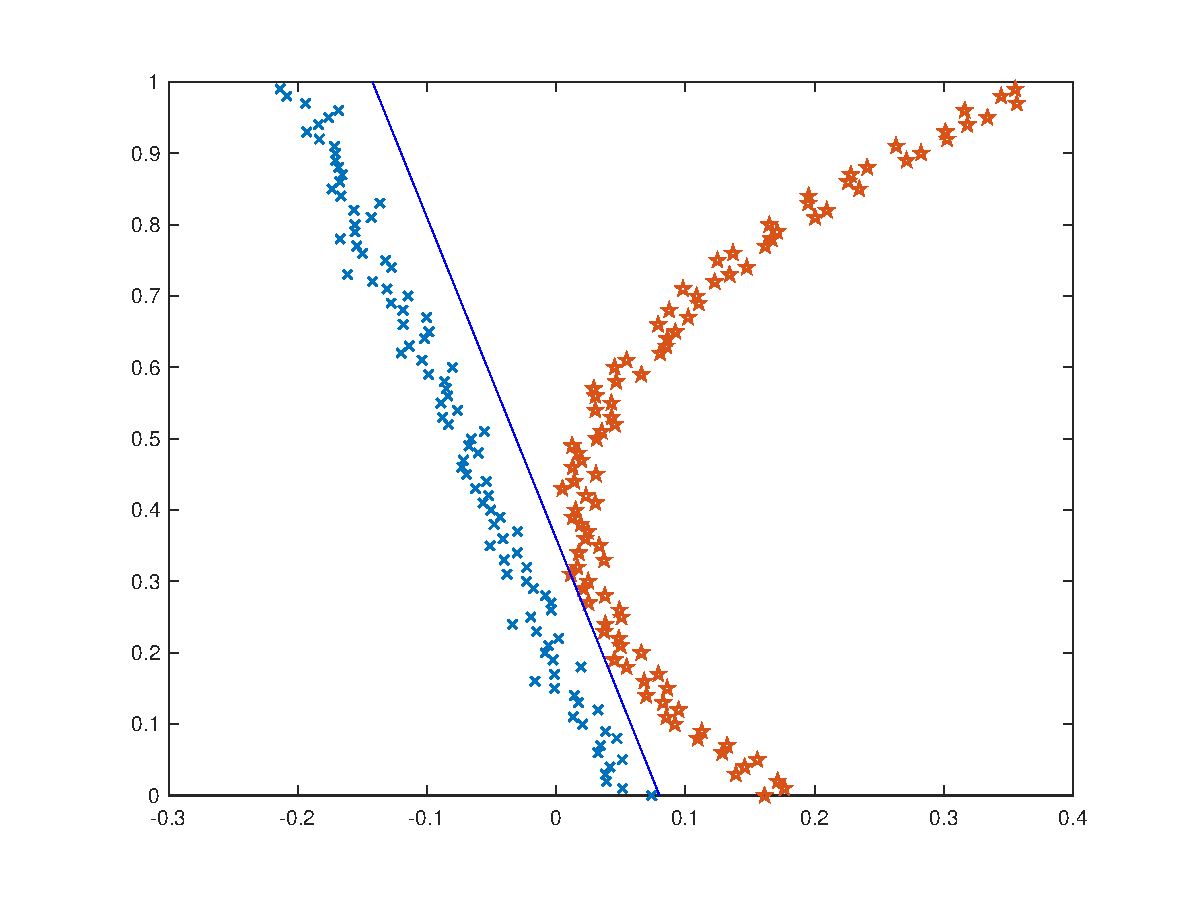
\includegraphics[width = .45\textwidth]{1_4}
\label{Fig.sub.2}
}
\end{figure}
\\
\begin{figure}[htbp]
\centering
\subfigure[d=15]{
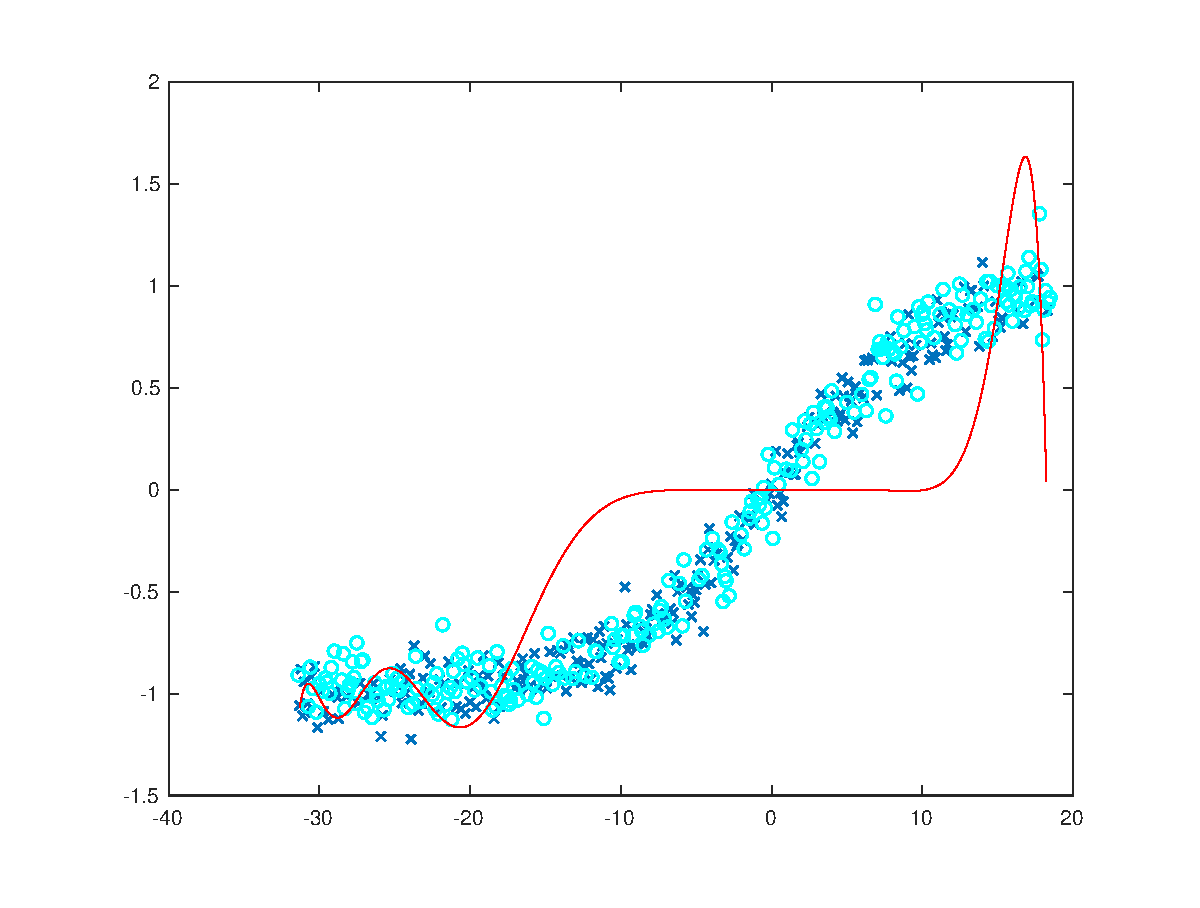
\includegraphics[width = .45\textwidth]{1_5}
}
\subfigure[d=20]{
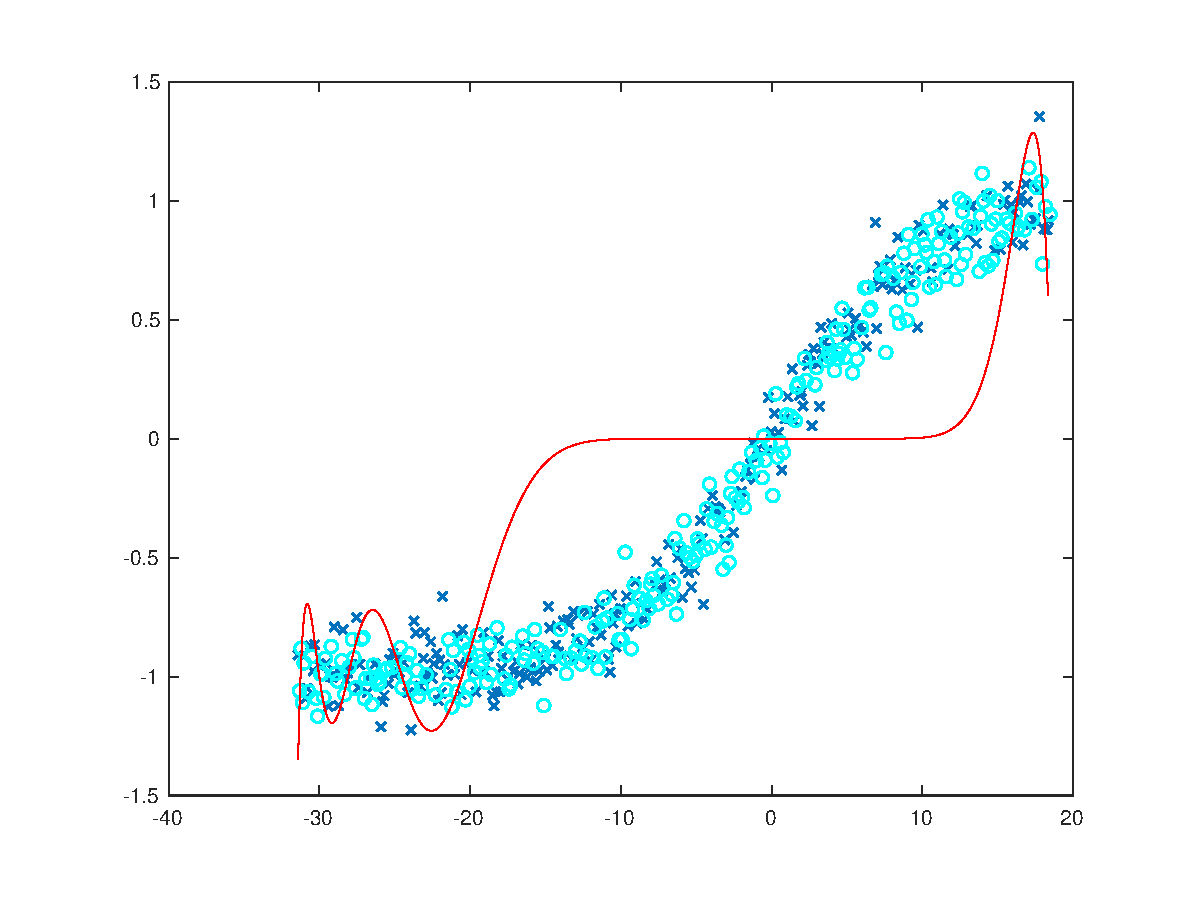
\includegraphics[width = .45\textwidth]{1_6}
}
\end{figure}
\\
Obviously the functions from \ref{Fig.sub.1} and \ref{Fig.sub.2} best fit the data set. Through cross-validation, we can get the best $d = 9$, which corresponds with the lowest loss on testing set,  as shown in \ref{Fig.sub.3} and \ref{Fig.sub.4}. 

The reason why training error keeps rising after $d = 10$ may be as we increase the polynomial degree, the disturbance between training examples becomes too large so that the coefficients explodes, making the training model unfit the training data.
\\
\begin{figure}[htbp]
\centering
\subfigure[cross-validation]{
\includegraphics[width = .45\textwidth]{1_7}
\label{Fig.sub.3}
}
\subfigure[overlaid]{
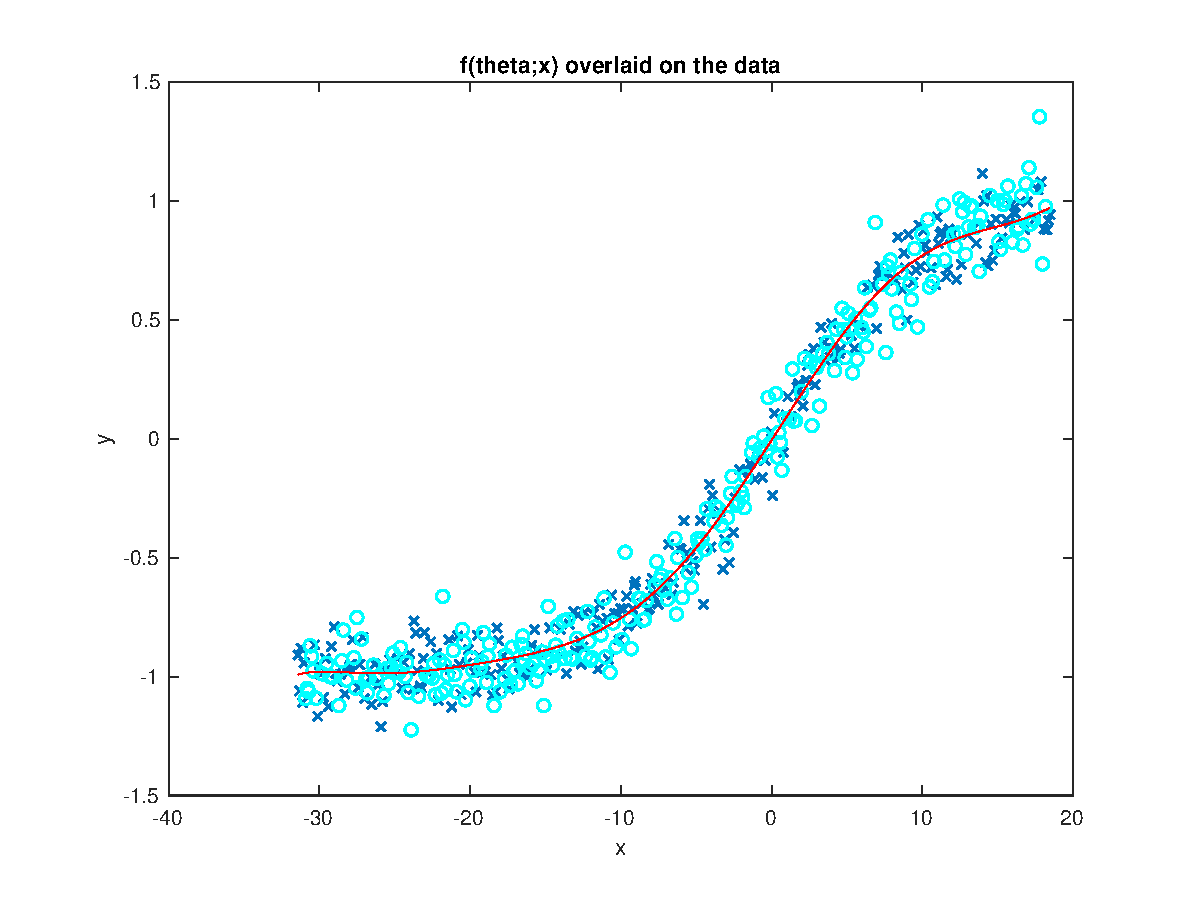
\includegraphics[width = .45\textwidth]{1_8}
\label{Fig.sub.4}
}
\end{figure}
\\

\section{Problem 2: logistic Regression}

For the function: 
\begin{align}
f(\textbf{x};\theta) = (1+\exp(-\theta^{\mathsf{T}}\textbf{x}))^{-1} \nonumber
\end{align}
with the loss function:
\begin{align}
L = (1-y_i)\log(1-f(x_i, \theta)) - y_i \log(f(x_i, \theta)) \nonumber
\end{align}

We were supposed to solve the gradient descent with derivation: $\nabla_{\theta}L = 0$

\begin{align}
\nabla_{\theta}L &= \frac{1}{N} \sum^{N}_{i=1} \left[\frac{(1-y_i)}{1-f(x_i; \theta)} - \frac{y_i}{f(x_i; \theta)} \right] f^{'}(x_i;\theta) \nonumber\\
& = \frac{1}{N} \sum^{N}_{i=1} \left[ \frac{(1-y_i)(1+e^{-\theta^{\mathsf{T}}x_i})}{e^{-\theta^{\mathsf{T}}x_i}}  - y_i(1+e^{-\theta^{\mathsf{T}}x_i}) \right] \frac{x_i e^{-\theta^{\mathsf{T}}x_i}}{(1+e^{-\theta^{\mathsf{T}}x_i})^2} \nonumber\\
& = \frac{1}{N} \sum^{N}_{i=1} \left[ \frac{(1-y_i)x_i}{1+e^{-\theta^{\mathsf{T}}x_i}} - \frac{y_i x_i e^{-\theta^{\mathsf{T}}x_i}}{1+e^{-\theta^{\mathsf{T}}x_i}}  \right] \nonumber \\
& = \frac{1}{N} \sum^{N}_{i=1} \left[  (1-y_i)x_i - y_i x_i e^{-\theta^{\mathsf{T}}x_i}\right] (1+e^{-\theta^{\mathsf{T}}x_i})^{-1}   \nonumber \\
& = \frac{1}{N} \sum^{N}_{i = 1} \left[   x_i -y_i x_i - y_i x_i (f(x_i; \theta)^{-1} - 1)\right]f(x_i; \theta)  \nonumber \\
& = \frac{1}{N} \sum^{N}_{i = 1} (  x_i f(x_i; \theta)- y_i x_i ) \nonumber 
\end{align}

However, this equation can't be solved analytically, only with recursive numerical method can we approach to the convex point. 

Using  GD, set the iteration to be 200000 with tolerance $\epsilon = 0.001$, step size $ \eta = 2 $,  the model will be as shown as $\ref{42(2)}$ and $\ref{42(1)}$.

The model obtained is $\theta = [ -26.5723, -117.8034, 9.0470]^{\top}$. Slightly change the tolerance as well as the step size, there's no notable difference regarding the convergence evolution rate and the model accuracy.

\begin{figure}[htbp]
\setcounter{subfigure}{8}
\centering
\subfigure[ error and risk ]{
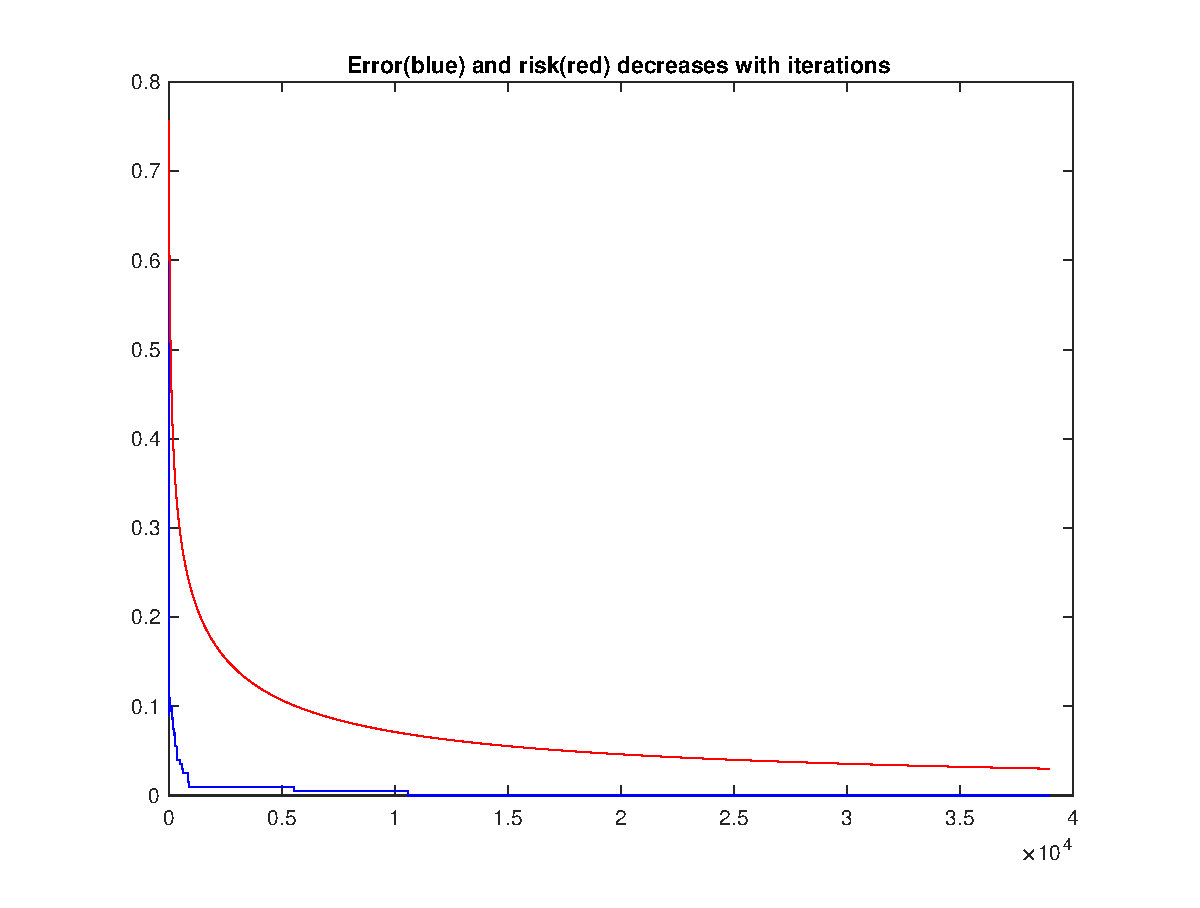
\includegraphics[width = .45\textwidth]{2_1}
\label{42(2)}
}
\subfigure[binary boundary]{
\includegraphics[width = .45\textwidth]{2_2}
\label{42(1)}
}
\end{figure}

Using SGD, set the batch size $b = 1$, step size $ \eta = 2 $,  the model will be as shown as $\ref{42(3)}$ and $\ref{42(4)}$.

The model obtained is $\theta = [ -11.9161, -58.4613, 4.3810]^{\top}$, which is quite the same as the previous one. increasing the batch size, the convergence rate will slow down a little, yet greater than GD.

\begin{figure}[htbp]
\setcounter{subfigure}{10}
\centering
\subfigure[ error and risk ]{
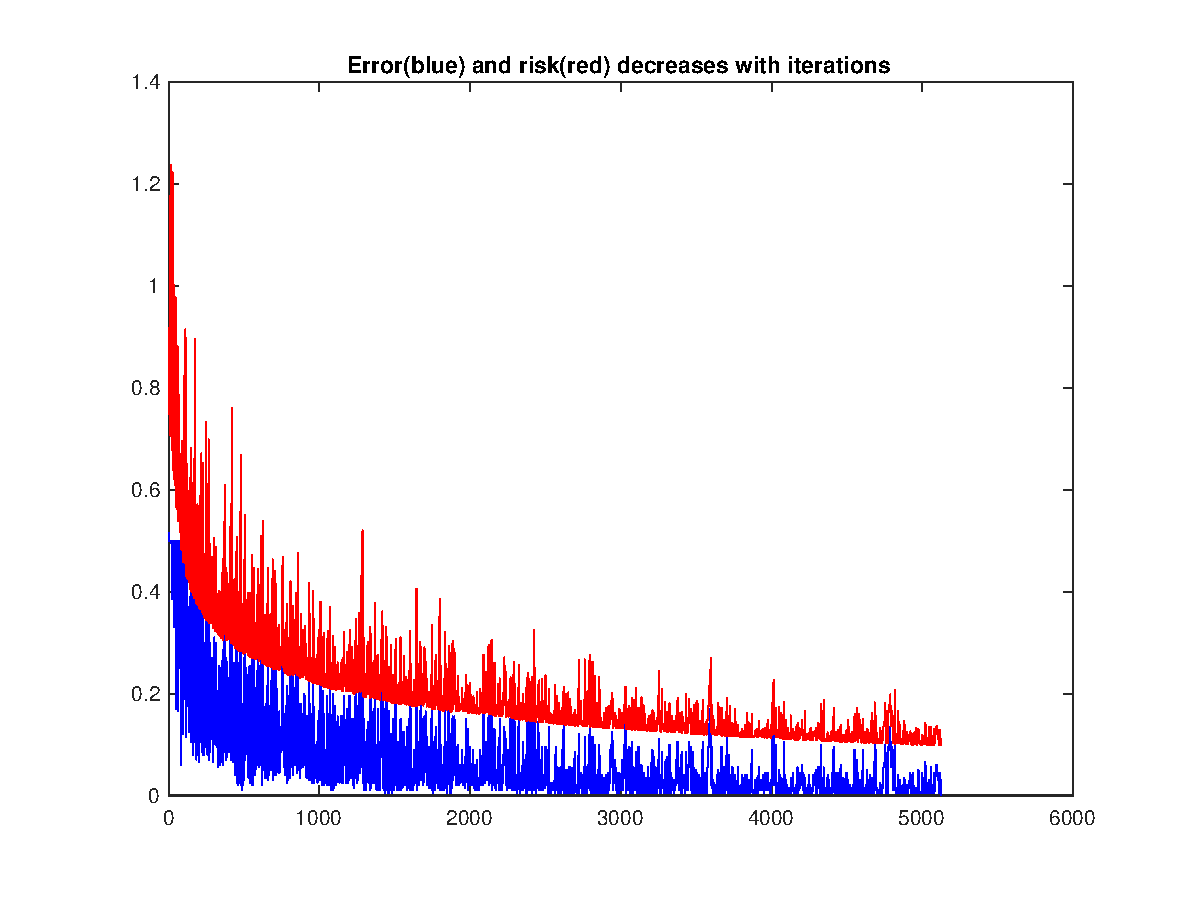
\includegraphics[width = .45\textwidth]{2_3}
\label{42(3)}
}
\subfigure[binary boundary]{
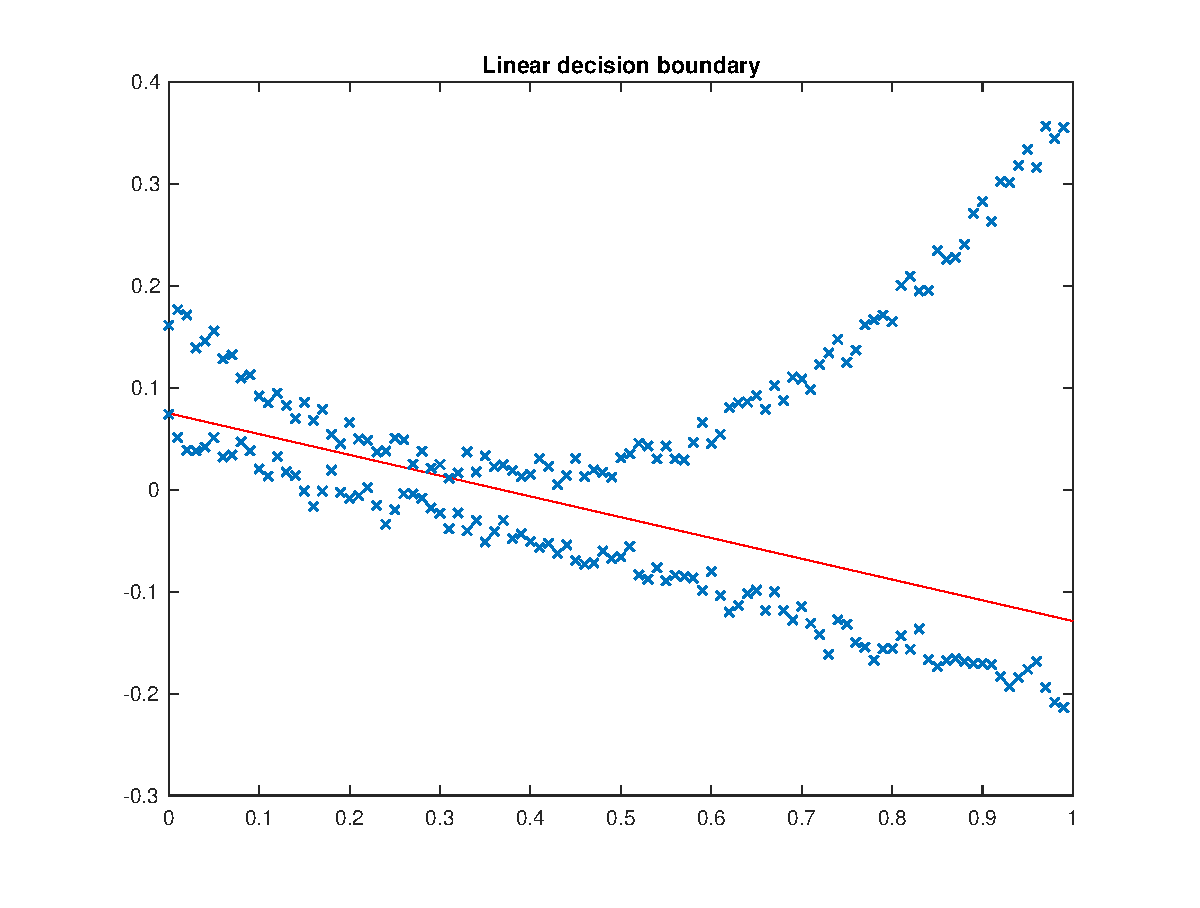
\includegraphics[width = .45\textwidth]{2_4}
\label{42(4)}
}
\end{figure}

Thus we conclude that SGD is more unstable while it converges faster than GD.

\section{problem 3: Multi-class Discrimination}

\subsection{a)}

In the 2-dimensional case, $K = 3$, suppose there are 2 functions $y_1(x)$ and $y_2(x)$, according to the rule, when $y_1(x)>0 \  \&\& \  y_2(x)>0$, the class of $x$ can be both $C_1$ or $C_2$, so it can't be determined, when $y_1(x)<0  \ \&\& \  y_2(x)<0$, we only know $x$ belongs to none of the 2 classes. Thus the approach leads to the ambiguous region x-space shown in $\ref{3_1}$ denoted by the orange area. Unless $y_1(x)$ and $y_2(x)$ are the same, otherwise there's always an ambiguous region

\begin{figure}[htbp]
\centering
\includegraphics[width = .7\textwidth]{../../../../Desktop/3_1.png}
\caption{}
\label{3_1}
\end{figure}

\subsection{b)}

According to the discrimination strategy, there are $K(K-1)/2 = 3$ linear functions when $k = 3$, which can be defined as follows:

\begin{align}
&y_{12}(x) > 0 \quad x \in C_1 \quad y_{12}(x) < 0 \quad x \in C_2 \quad \nonumber \\
&y_{13}(x) > 0 \quad x \in C_1 \quad y_{12}(x) < 0 \quad x \in C_3 \quad \nonumber \\
&y_{23}(x) > 0 \quad x \in C_2 \quad y_{12}(x) < 0 \quad x \in C_3 \quad \nonumber 
\end{align}

the structure is not well-defined because of following paradox:

\begin{align}
&y_{12}(x) > 0 \ \&\& \ y_{13}(x) < 0  \quad x \in C_1 \ \&\& \ x\in C_3  \nonumber \\
&y_{13}(x) > 0 \ \&\& \ y_{23}(x) < 0  \quad x \in C_1 \ \&\& \ x\in C_2 \nonumber \\
&y_{23}(x) > 0 \ \&\& \ y_{13}(x) < 0 \quad x \in C_2 \ \&\& \ x\in C_3  \nonumber \\
&y_{12}(x) > 0 \ \&\& \ y_{13}(x) < 0  \ \&\& \ y_{23}(x) > 0 \quad x \in C_1 \ \&\& \ x\in C_3 \ \&\&\ x\in C_2  \nonumber 
\end{align}

Which leads to the ambiguous region in $\ref{3_2}$:

\begin{figure}[htbp]
\centering
\includegraphics[width = .7\textwidth]{../../../../Desktop/3_2.png}
\caption{}
\label{3_2}
\end{figure}


\end{document}